%----------------------------------------------------------------------------------------
%	PACKAGES AND OTHER DOCUMENT CONFIGURATIONS
%----------------------------------------------------------------------------------------

	\documentclass[a4paper, 11pt, oneside]{book}

	\usepackage[sc]{mathpazo} % Use the Palatino font
	\usepackage[spanish, es-tabla]{babel}
	\usepackage[utf8]{inputenc}
	\usepackage{lipsum}
	\usepackage{graphicx}
	\usepackage[T1]{fontenc} % Use 8-bit encoding that has 256 glyphs
	\linespread{1.15} % Line spacing - Palatino needs more space between lines
	%\usepackage{microtype} % Slightly tweak font spacing for aesthetics
	%
	\usepackage[hmarginratio=1:1,left=20mm, top=32mm,columnsep=20pt]{geometry} % Document margins
	%\usepackage{multicol} % Used for the two-column layout of the document
	%\usepackage[hang, small,labelfont=bf,up,textfont=it,up]{caption} % Custom captions under/above floats in tables or figures
	%\usepackage{mathtools}
	%\usepackage{booktabs} % Horizontal rules in tables
	\usepackage{float} % Required for tables and figures in the multi-column environment - they need to be placed in specific locations with the [H] (e.g. \begin{table}[H])
	\usepackage{hyperref} % For hyperlinks in the PDF
	\usepackage{appendix}
	%\usepackage{wrapfig}
	%%\usepackage[]{mcode} % For embebing matlab code
	%\usepackage[makeroom]{cancel}
	%
	%%\usepackage{lettrine} % The lettrine is the first enlarged letter at the beginning of the text
	%\usepackage{paralist} % Used for the compactitem environment which makes bullet points with less space between them
	%
	\usepackage{abstract} % Allows abstract customization
	\renewcommand{\abstractnamefont}{\normalfont\bfseries} % Set the "Abstract" text to bold
	\renewcommand{\abstracttextfont}{\normalfont\small\itshape} % Set the abstract itself to small italic text
	%%
	%\usepackage{titlesec} % Allows customization of titles
	%%\renewcommand\thesection{\Roman{section}} % Roman numerals for the sections
	%%\renewcommand\thesubsection{\Roman{subsection}} % Roman numerals for subsections
	%\titleformat{\section}[block]{\large\scshape\centering}{\thesection.}{1em}{} % Change the look of the section titles
	%\titleformat{\subsection}[block]{\large\centering}{\thesubsection.}{1em}{} % Change the look of the section titles
	%
	%\usepackage{fancyhdr} % Headers and footers
	%\pagestyle{fancy} % All pages have headers and footers
	%\fancyhead{} % Blank out the default header
	%\fancyfoot{} % Blank out the default footer
	%\fancyhead[C]{Titulo Corto% based on TRACS 
	%\hspace{4pt} $\bullet$ \hspace{4pt} MES ANO } % Custom header text
	%\fancyfoot[RO,LE]{\thepage} % Custom footer text
	%
	\usepackage{cite}
	\usepackage{listings}
	\usepackage{color}

	\graphicspath{{../Graphics/}}
	%
	%\DeclareGraphicsExtensions{.pdf,.png,.jpg} % Graphics type

%----------------------------------------------------------------------------------------
%	   METADATA
%----------------------------------------------------------------------------------------

	%\title{
	%	\selectfont\textbf{TITULO}% Article title
	%}
%
	%\author{
	%	\textsc{Jaime Diez Gonzalez-Pardo}\\
	%	%\thanks{A thank you or further information}\\ % Your name
	%	\fontsize{28pt}{10pt} Universidad de Cantabria \\ % Your institution
	%	%\thanks{A thank you or further information}\\[2mm] % Your name
	%	\normalsize gsdfgdfgdfgatura \\ 
	%	\normalsize{Compañeros:} \textsc{NOMBRE COMPANEROS }\\
	%	%\vspace{5mm}
	%}
%
	%\date{\today}

%----------------------------------------------------------------------------------------
%      · DOCUMENT
%----------------------------------------------------------------------------------------

	\begin{document}

		\begin{titlepage} 

			\newcommand{\HRule}{\rule{\linewidth}{0.5mm}} 
			
			\center % Centre everything on the page
			
			%------------------------------------------------
			%	Headings
			%------------------------------------------------
			
				%------------------------------------------------
				%	Logo
				%------------------------------------------------
				
					\begin{figure}[H]
						\centering
						
\includegraphics[scale=0.6]{download.png}
					\end{figure}

					\textsc{\LARGE Facultad de Ciencias}\\[1.5cm] 
			
			
			%------------------------------------------------
			%	Title
			%------------------------------------------------
			
				\HRule\\[0.4cm]
				
				{\huge\bfseries Simulación de peines de frecuencia óptica generados por láseres de semiconductor}\\[0.8cm] % Title of your document

				{\huge Simulation of optical frequecy comb generate by semiconductor lasers}\\[0.4cm] % Title of your document
				
				\HRule\\[1.5cm]

				{\Large Trabajo de Fin de Grado para acceder al}\\[0.4cm]

				{\LARGE\bfseries Grado en Física}\\[3cm]
			
			%------------------------------------------------
			%	Author(s)
			%------------------------------------------------
			
				\begin{flushright}
					\large
					\textit{Autor}\\
					Jaime \textsc{DÍEZ GONZÁLEZ-PARDO} \\ % Your name
					\large
					\textit{Director}\\
					Dr. Á.A. \textsc{VALLE GUTIERREZ} % Supervisor's name
				\end{flushright}
			
			%------------------------------------------------
			%	Date
			%------------------------------------------------
			
				\vfill\vfill\vfill % Position the date 3/4 down the remaining page
				
				{\large\today} % Date, change the \today to a set date if you want to be precise
				
			%----------------------------------------------------------------------------------------
			
				\vfill % Push the date up 1/4 of the remaining page
		
		\end{titlepage}

		\abstract{
			\addtocontents{toc}{\vspace{1em}}  % Add a gap in the Contents, for aesthetics

				Hola

		}

		\renewcommand{\abstractname}{Abstract}

		\abstract{
			\addtocontents{toc}{\vspace{1em}}  % Add a gap in the Contents, for aesthetics

				Hola

		}

		%\thispagestyle{fancy} % All pages have headers and footers

		\tableofcontents

		\listoffigures

		%----------------------------------------------------------------------------------------
		%	  ARTICLE CONTENTS
		%----------------------------------------------------------------------------------------

			\addtocontents{toc}{\vspace{0.1cm}}
			\chapter{Introducción} % Scope of the project = rad effects + minimization
				\label{sec:Intro}

				%\input{}

				\addtocontents{toc}{\vspace{0.1cm}}
				\section{Láseres de Semiconductor}
					
					%\input{}

				\addtocontents{toc}{\vspace{0.1cm}}
				\section{Procesos Estocásticos}
					
					%\input{}

				\addtocontents{toc}{\vspace{0.1cm}}
				\section{Dinámica No Lineal}
					
					%\input{}
%
				\addtocontents{toc}{\vspace{0.1cm}}
				\section{Peines de Frecuencia Óptica}
					
					
Que son, caracteristicas principales y como se generan,...

	\subsection{\textit{Gain-Switching}}

		hola que tal todos

	\subsection{Inyección Ópticar}

		adios a todos 

	\subsection{Aplicaciones}




				\addtocontents{toc}{\vspace{0.1cm}}
				\section{Objetivo del Estudio}
					
					%\input{}
				
			\addtocontents{toc}{\vspace{0.1cm}}
			\chapter{Modelo Computacional}

				\addtocontents{toc}{\vspace{0.1cm}}
				\section{RoF}
				
					%\input{}

				\addtocontents{toc}{\vspace{0.1cm}}
				\section{Código de la Simulación}
				
					%\input{}
				
			\addtocontents{toc}{\vspace{0.1cm}}
			\chapter{OFC (Gain Switching)}

				\graphicspath{{$HOME/TFG/Graphics/Cpt1-Charactz/}}

		\begin{figure}[H]
			\centering
			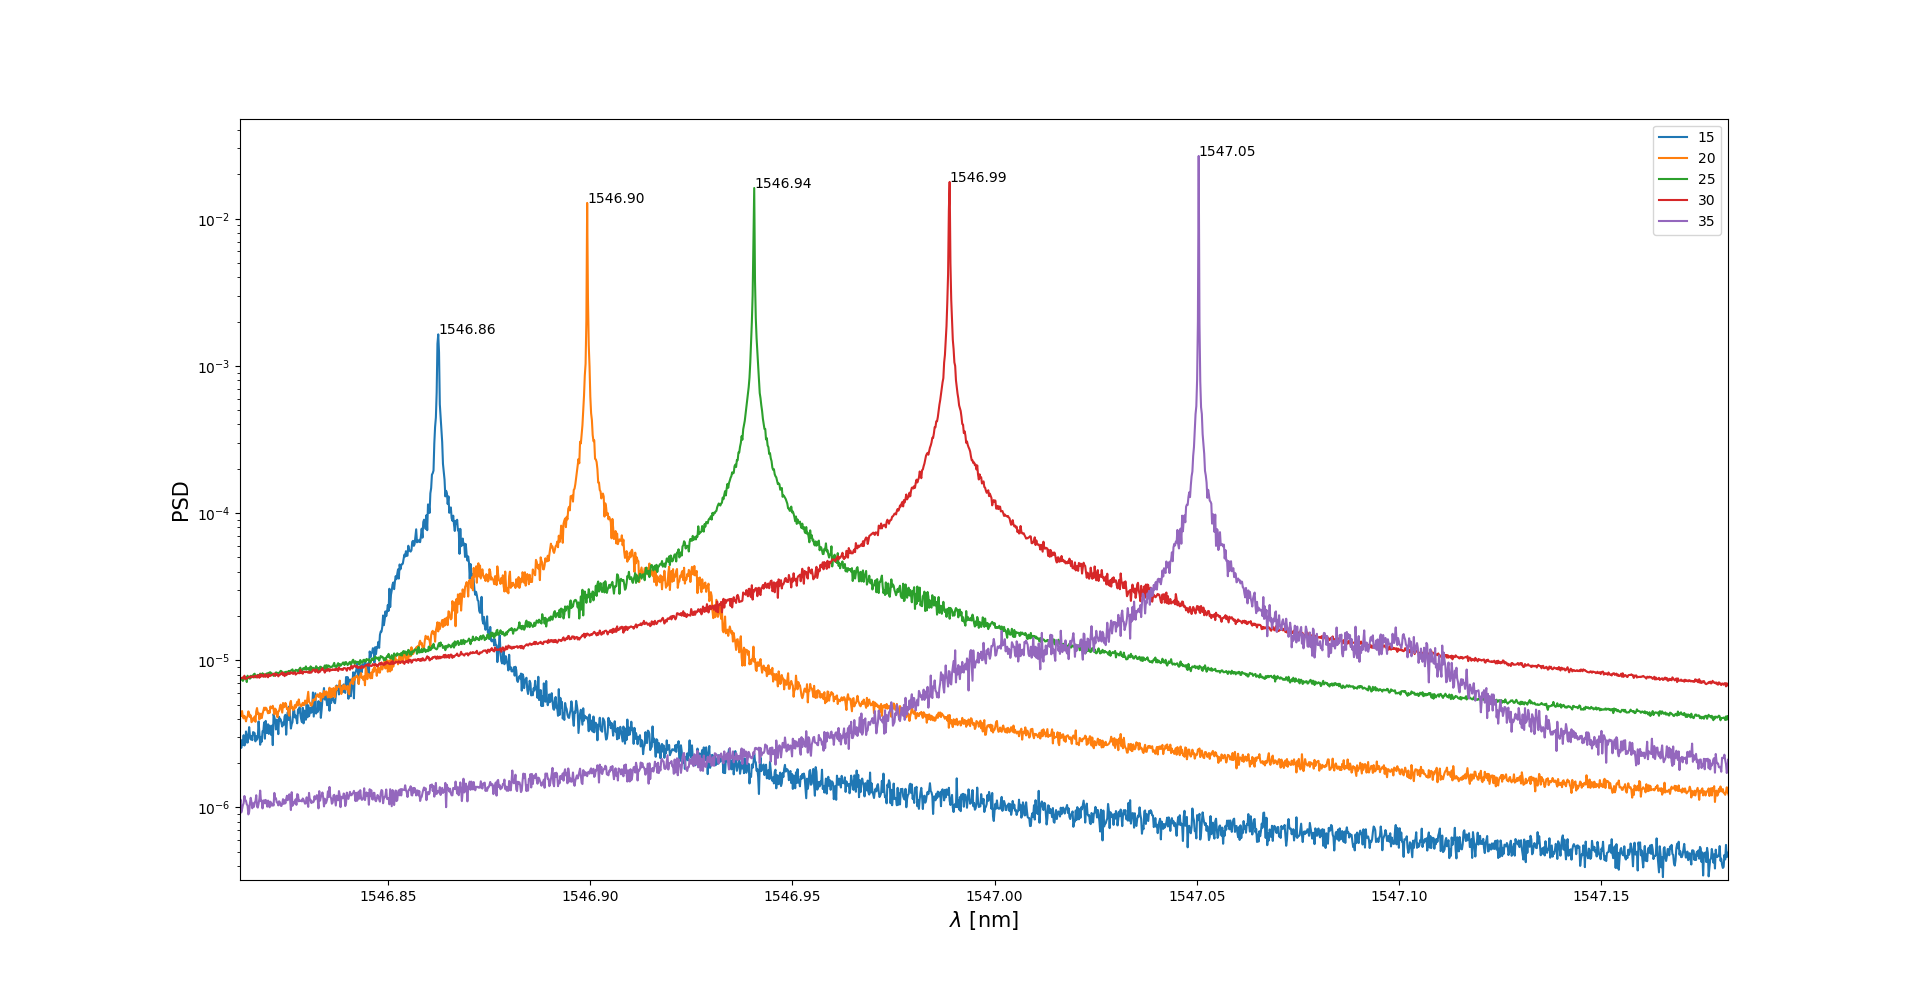
\includegraphics[width=1.0\linewidth]{Espectros.png}
			\caption{\label{Img:widgets}Espectros en continua de la simulacion}
		\end{figure}

		\begin{table}[H]
			\centering
			\begin{tabular}{c c}
				\hline
				$I_{Bias}$ & $\lambda$ \\\hline 
				15 & 1546.86 \\
				20 & 1546.90 \\
				25 & 1546.94 \\
				30 & 1546.99 \\
				35 & 1547.05 \\\hline
			\end{tabular}
			\caption{\label{tab:label}Lambdas de la simulacion}
		\end{table}

		\begin{figure}[H]
			\centering
			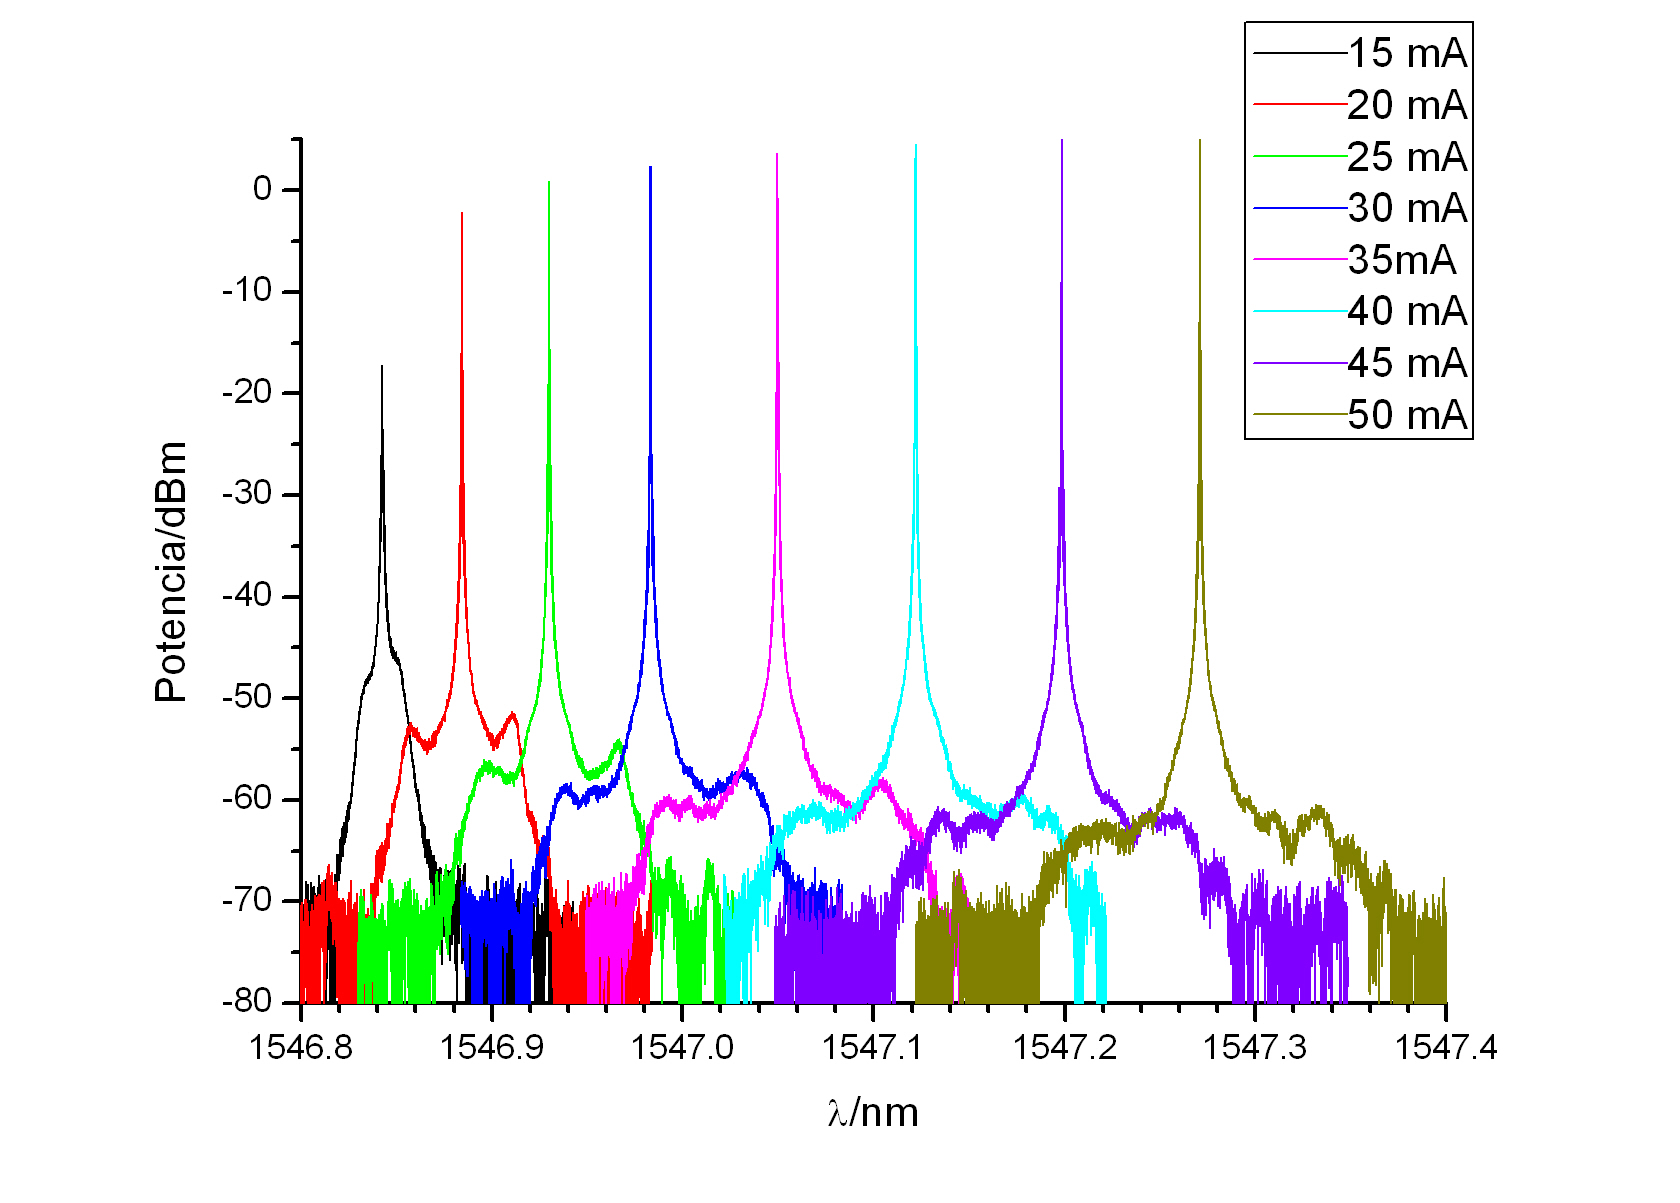
\includegraphics[width=1.0\linewidth]{../Chaves/OFC-GS/EspectrosT25.jpg}
			\caption{\label{fig:EspectrosT25}Espectros en continua de Chaves}	
		\end{figure}
	

		\begin{figure}[H]
			\centering
			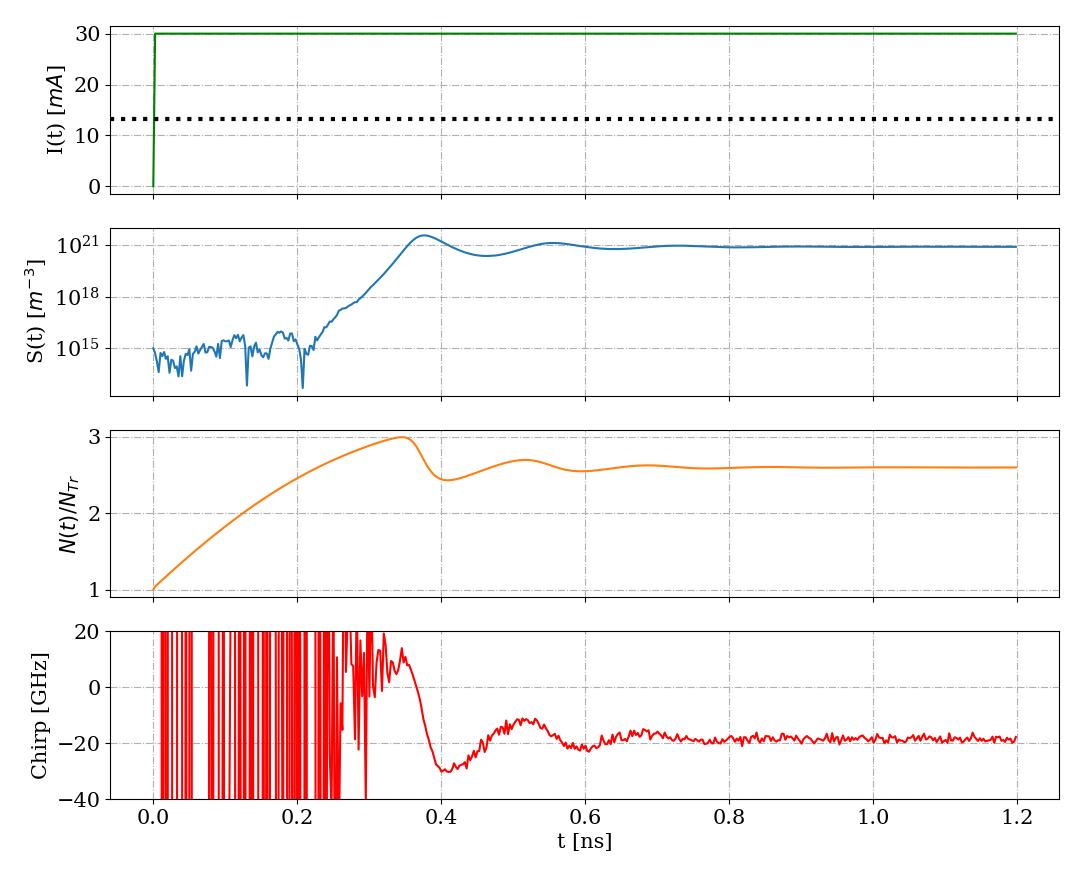
\includegraphics[width=1.0\linewidth]{transitorio.png}
			\caption{\label{fig:transitorio}Transitorio}	
		\end{figure}

		\begin{figure}[H]
			\centering
			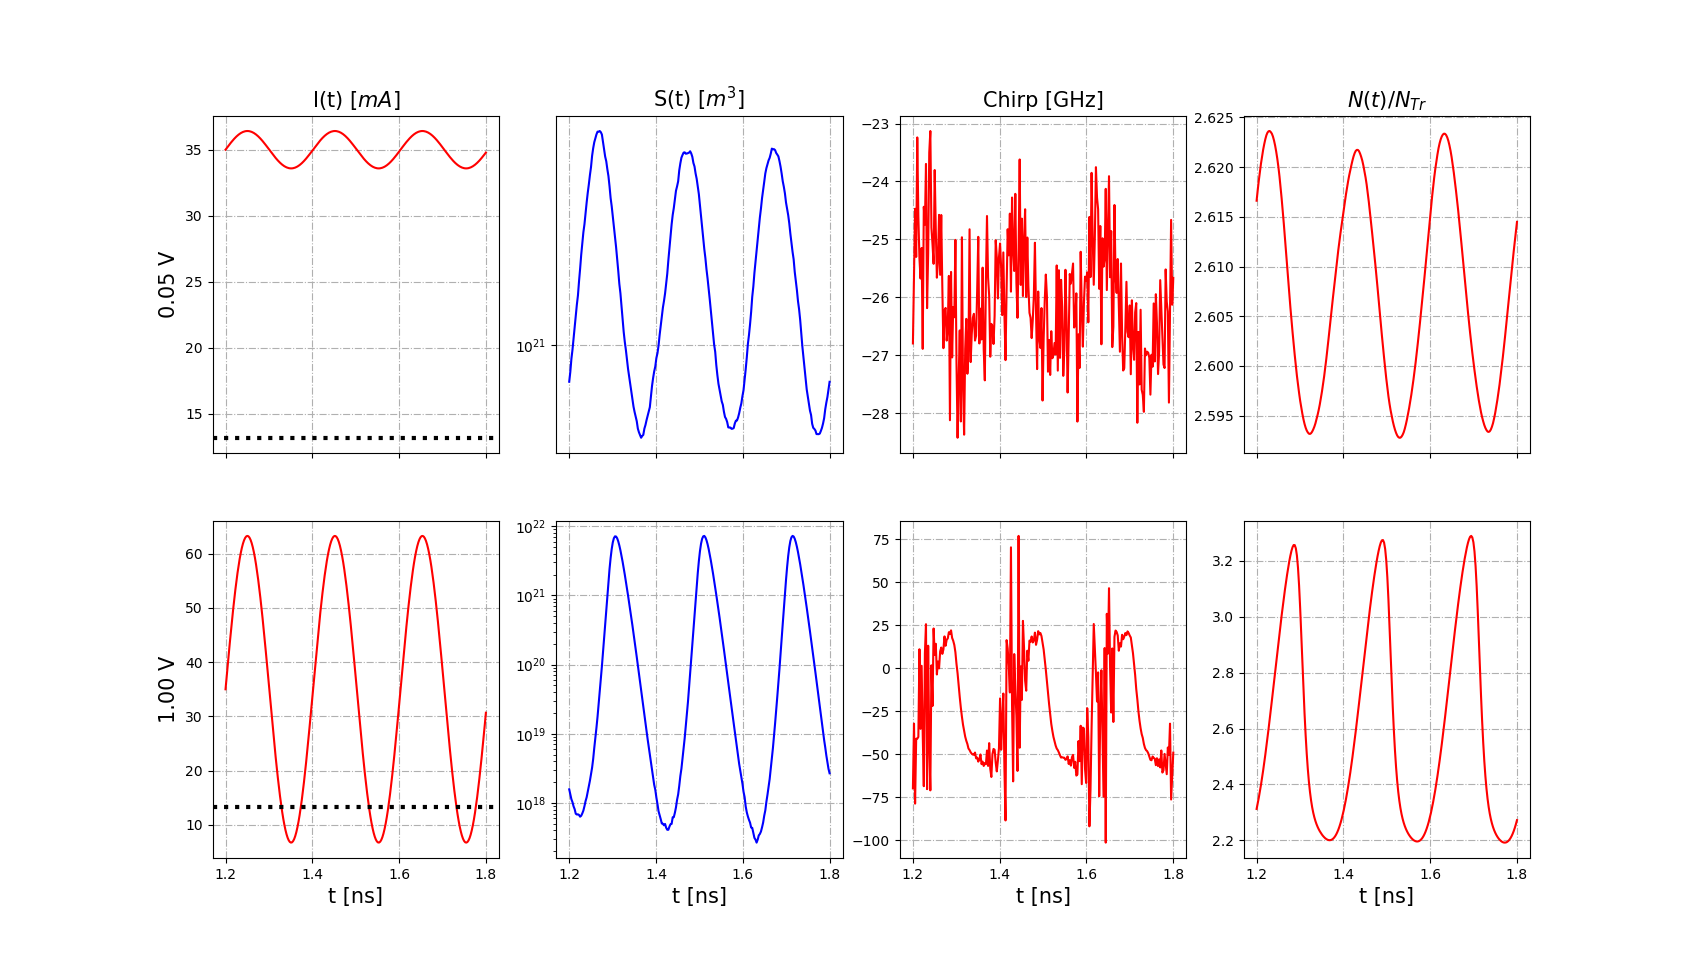
\includegraphics[width=1.0\linewidth]{rateEquations.png}
			\caption{\label{fig:rateEquations}RateEquations}	
		\end{figure}

		\begin{figure}[H]
			\centering
			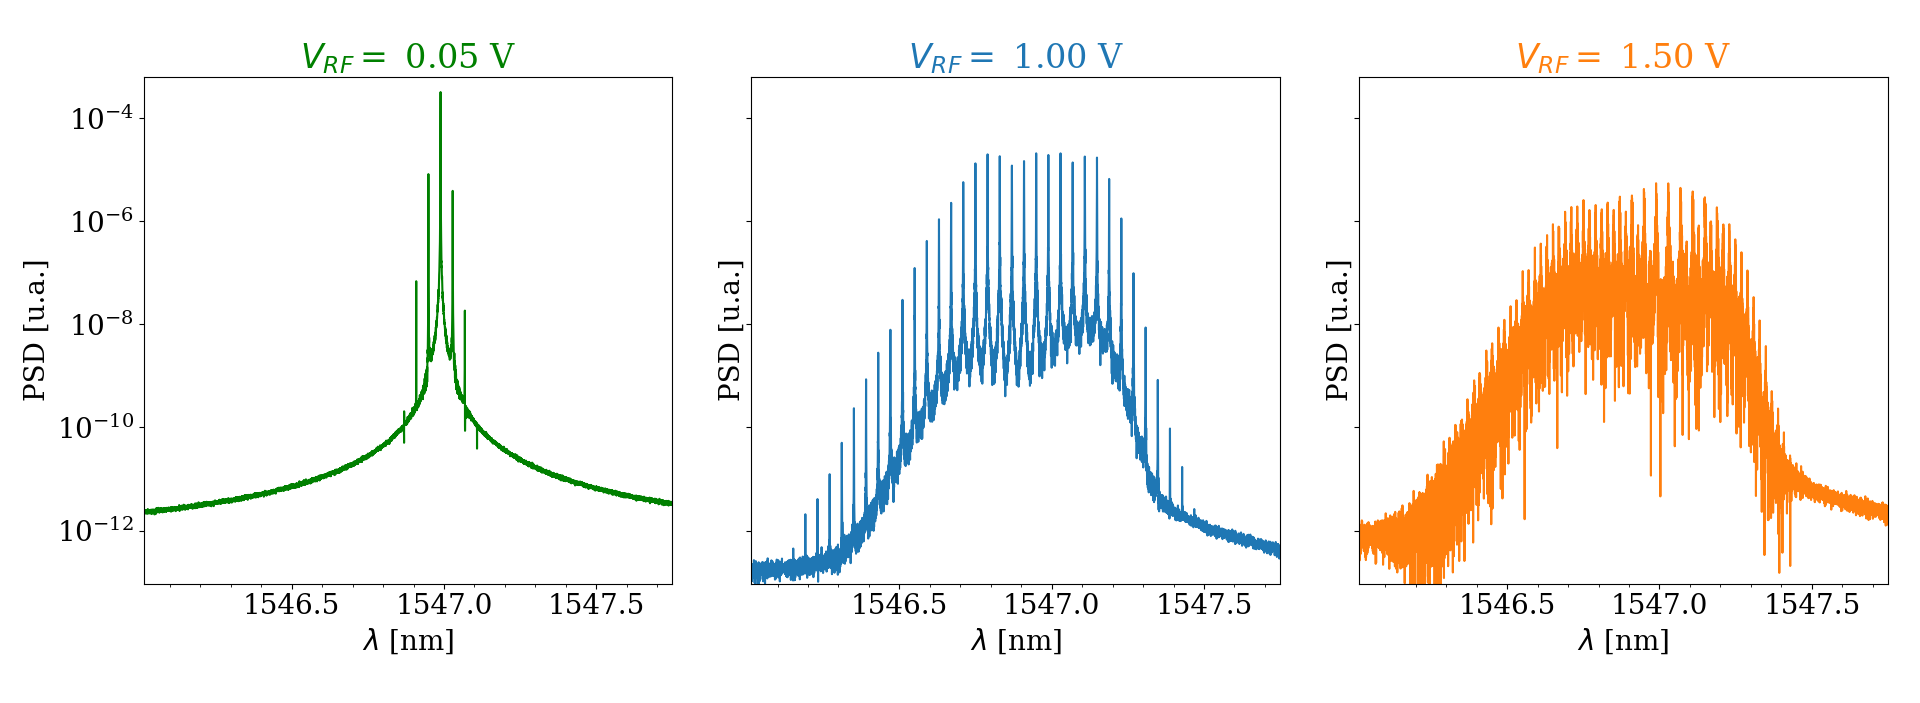
\includegraphics[width=1.0\linewidth]{PSD.png}
			\caption{\label{fig:PSD}PSD}	
		\end{figure}

		\begin{figure}[H]
			\centering
			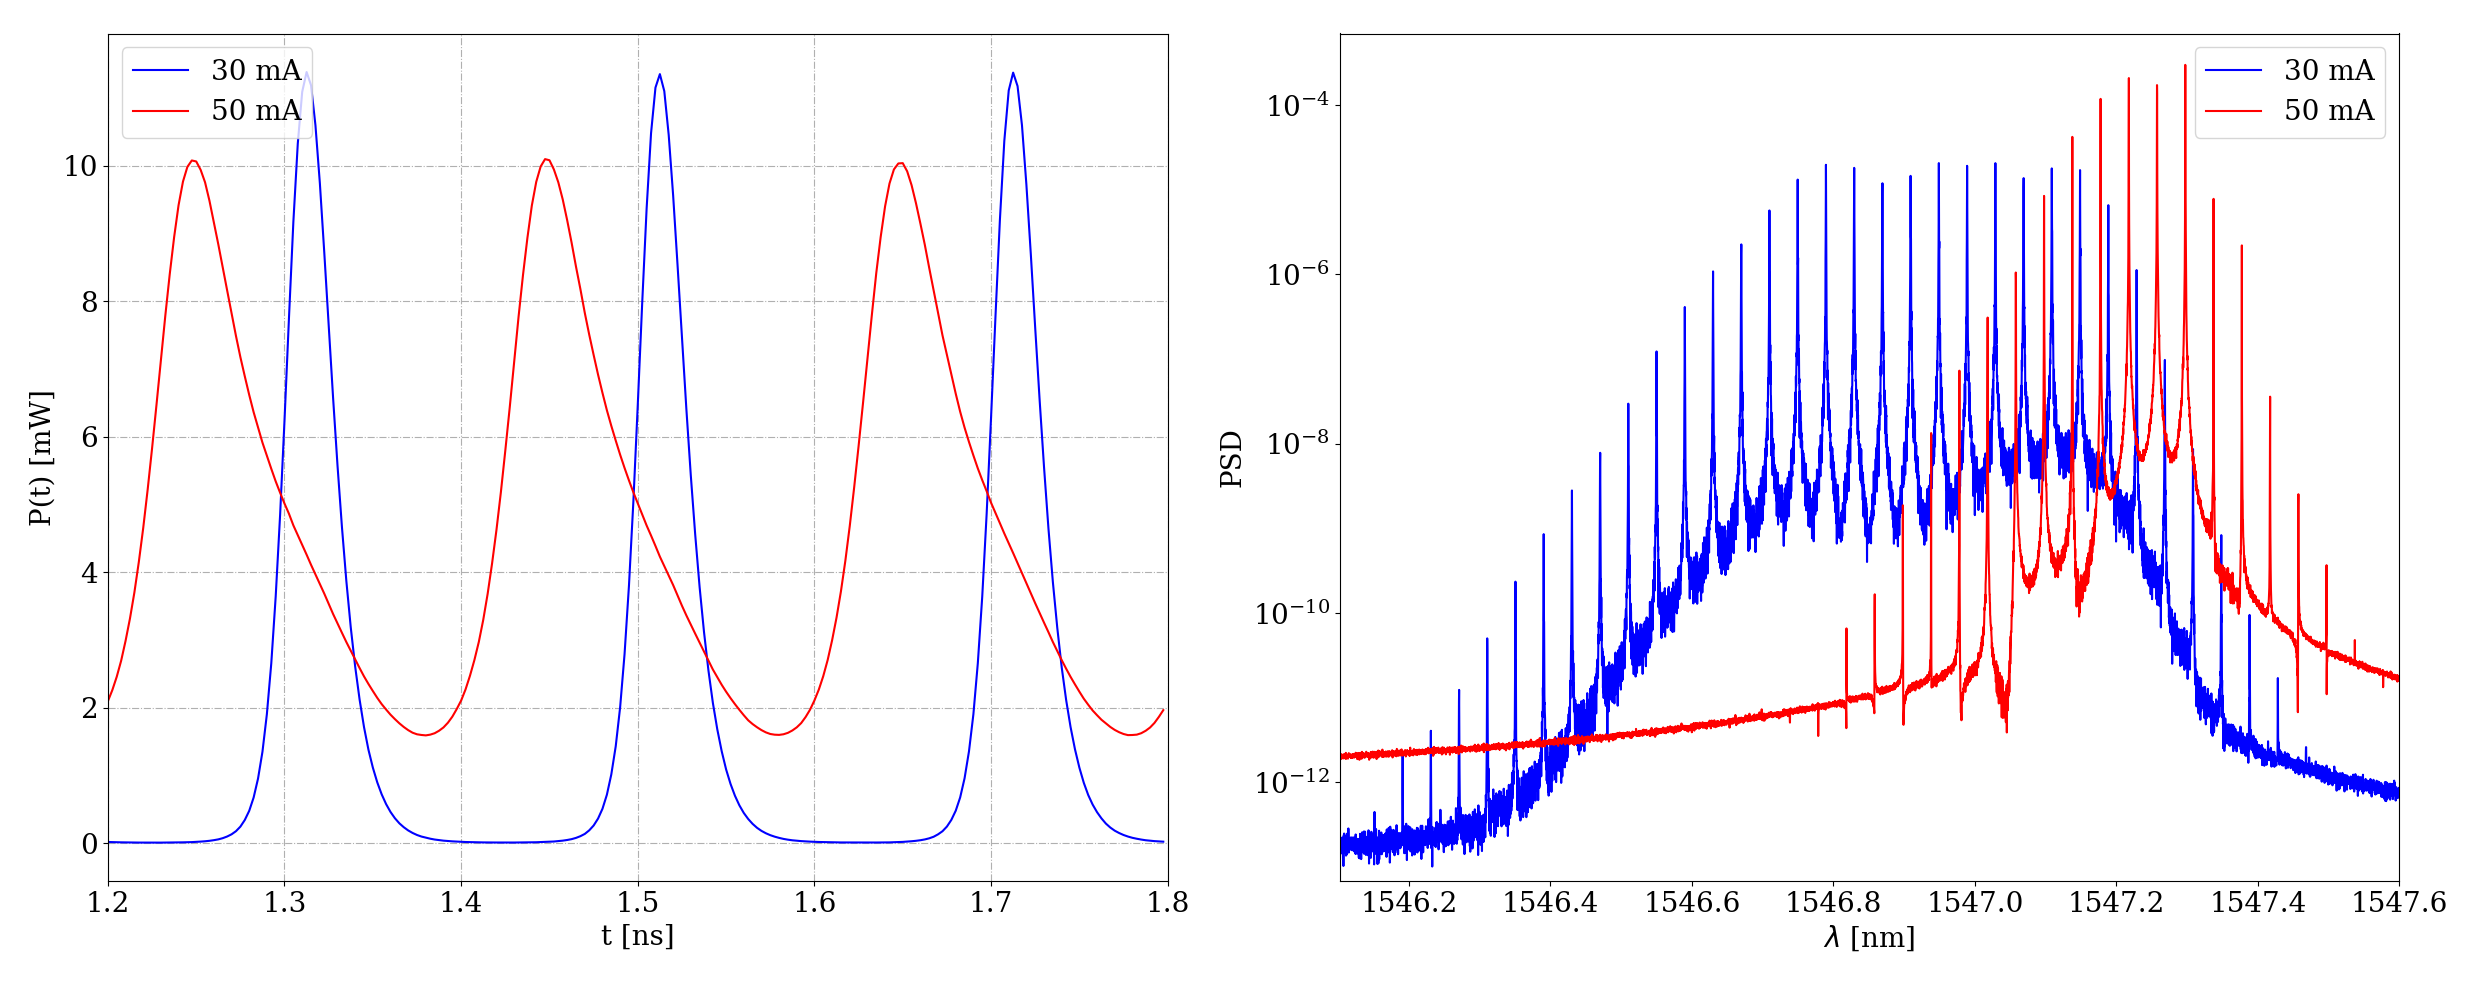
\includegraphics[width=1.0\linewidth]{current.png}
			\caption{\label{fig:current}Current}	
		\end{figure}

		\begin{figure}[H]
			\centering
			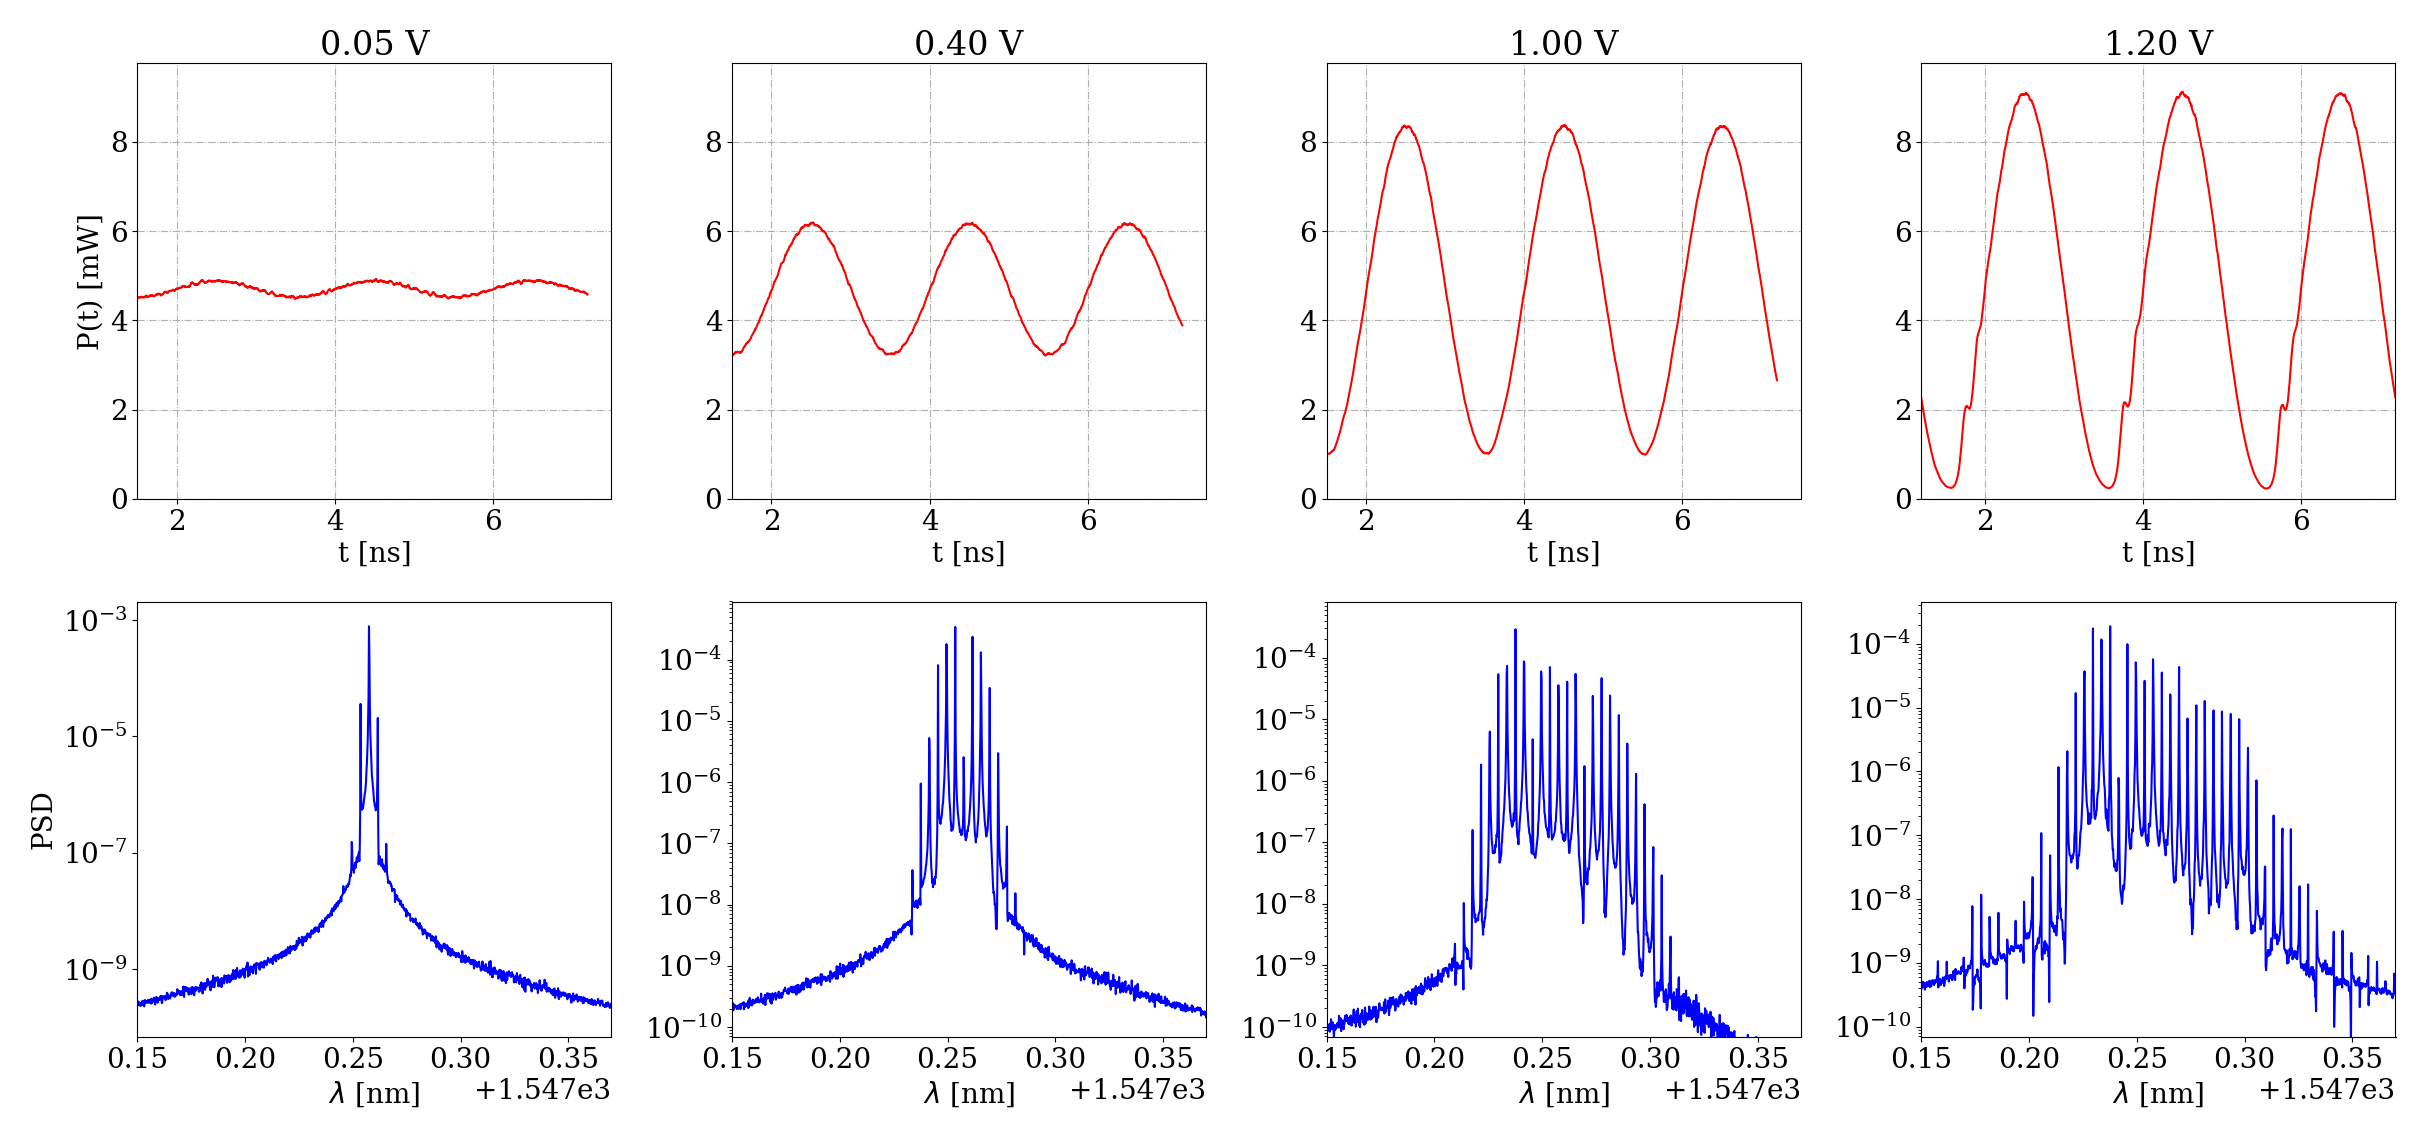
\includegraphics[width=1.0\linewidth]{500.png}
			\caption{\label{fig:500}500}	
		\end{figure}

		\begin{figure}[H]
			\centering
			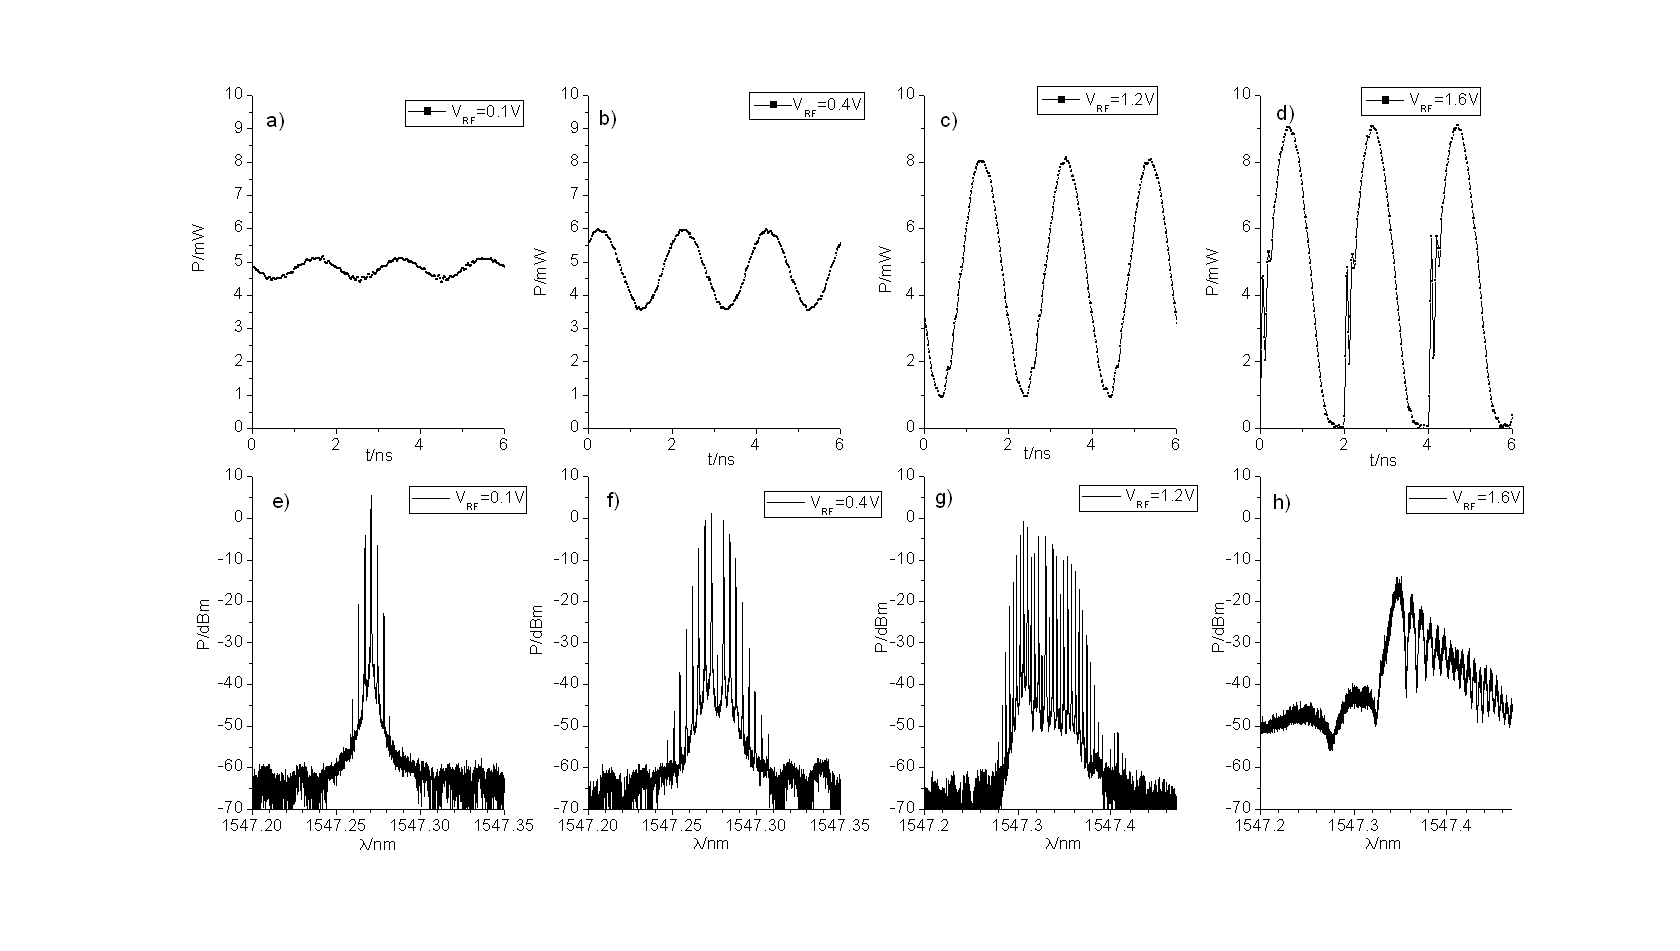
\includegraphics[width=1.0\linewidth]{../Chaves/OFC-GS/500mhz.png}
			\caption{\label{fig:500mhz}500mhz}	
		\end{figure}
	

			\addtocontents{toc}{\vspace{0.1cm}}
			\chapter{Inyeccion de Luz}

				\graphicspath{{../Graphics/Cpt2-InjectCW/}}


			\begin{figure}[H]
				\centering
				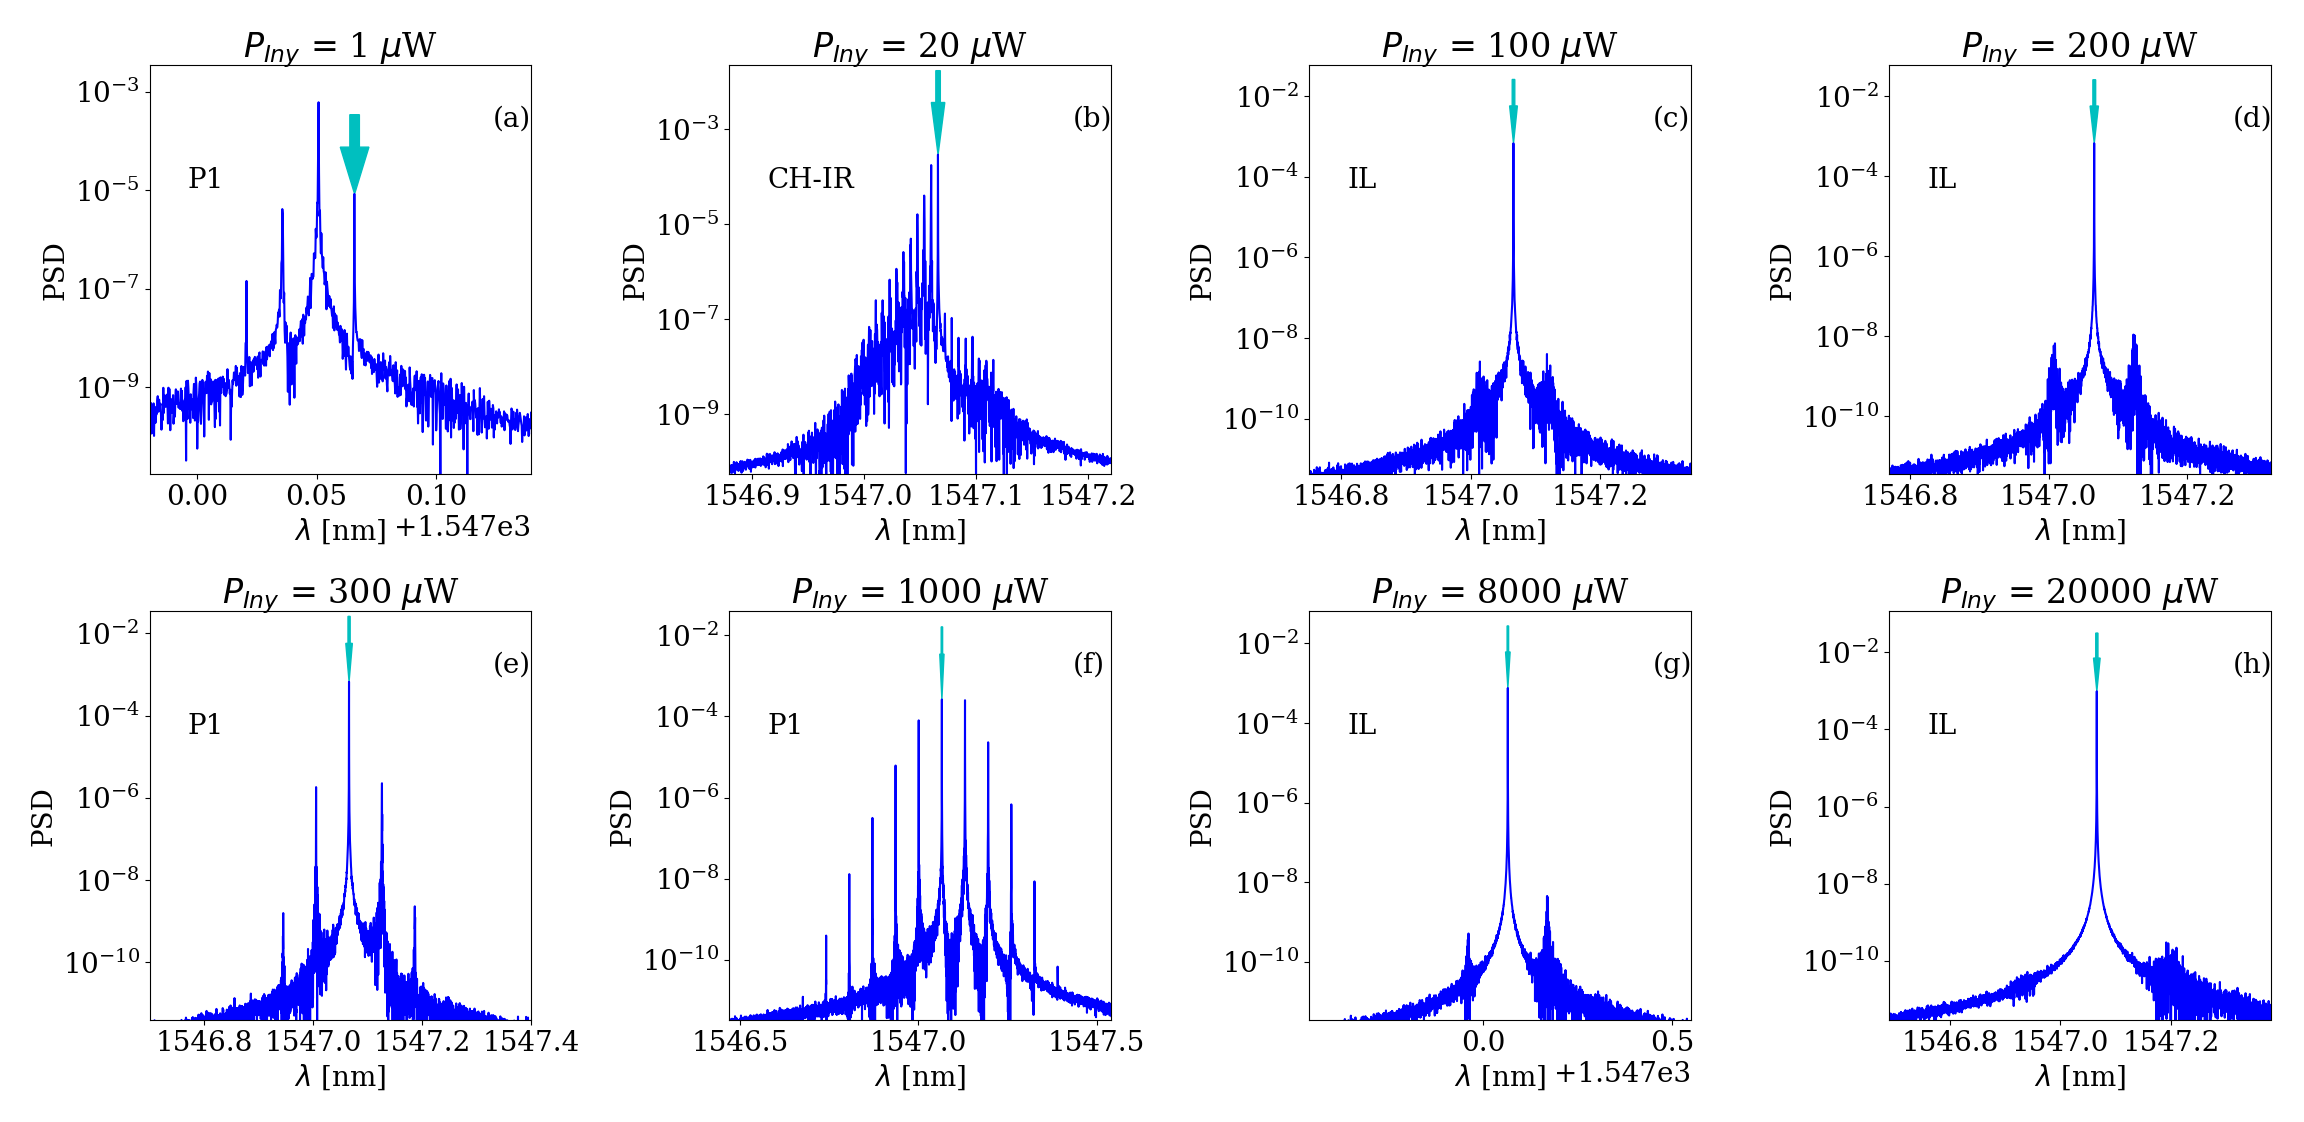
\includegraphics[width=1.0\linewidth]{zoneMap.png}
				\caption{\label{Img:widgets}el pie de pagina que le quieras 	poner a la imagen}
			\end{figure}

			\begin{figure}[H]
				\centering
				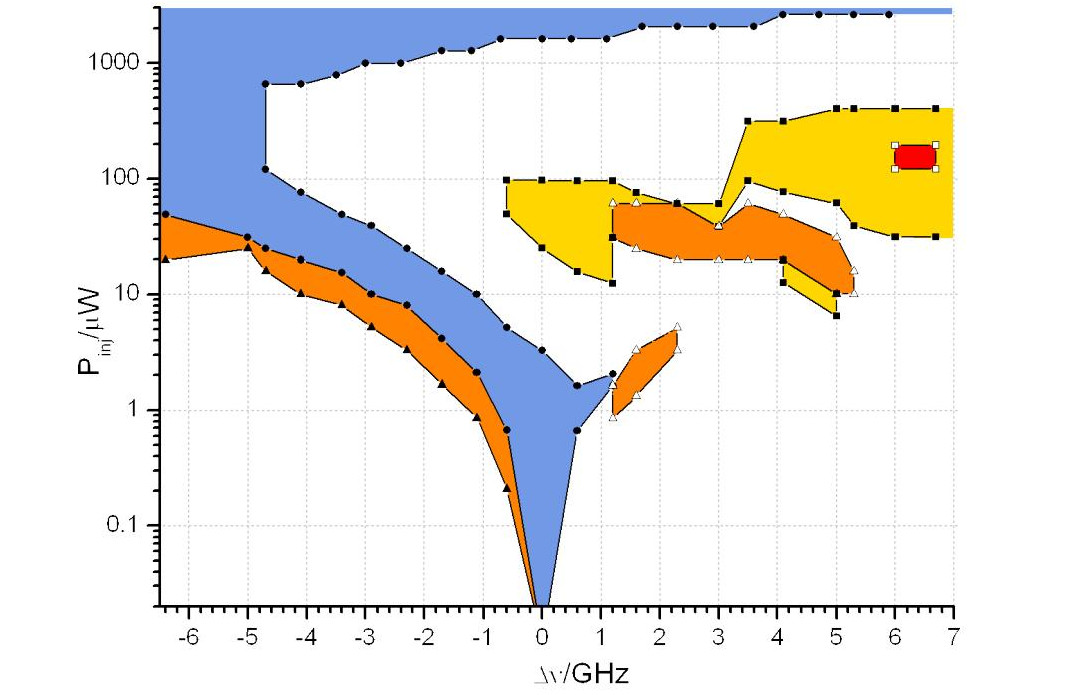
\includegraphics[width=1.0\linewidth]{mapa.jpg}
				\caption{\label{fig:map}Map}	
			\end{figure}

			\begin{figure}[H]
				\centering
				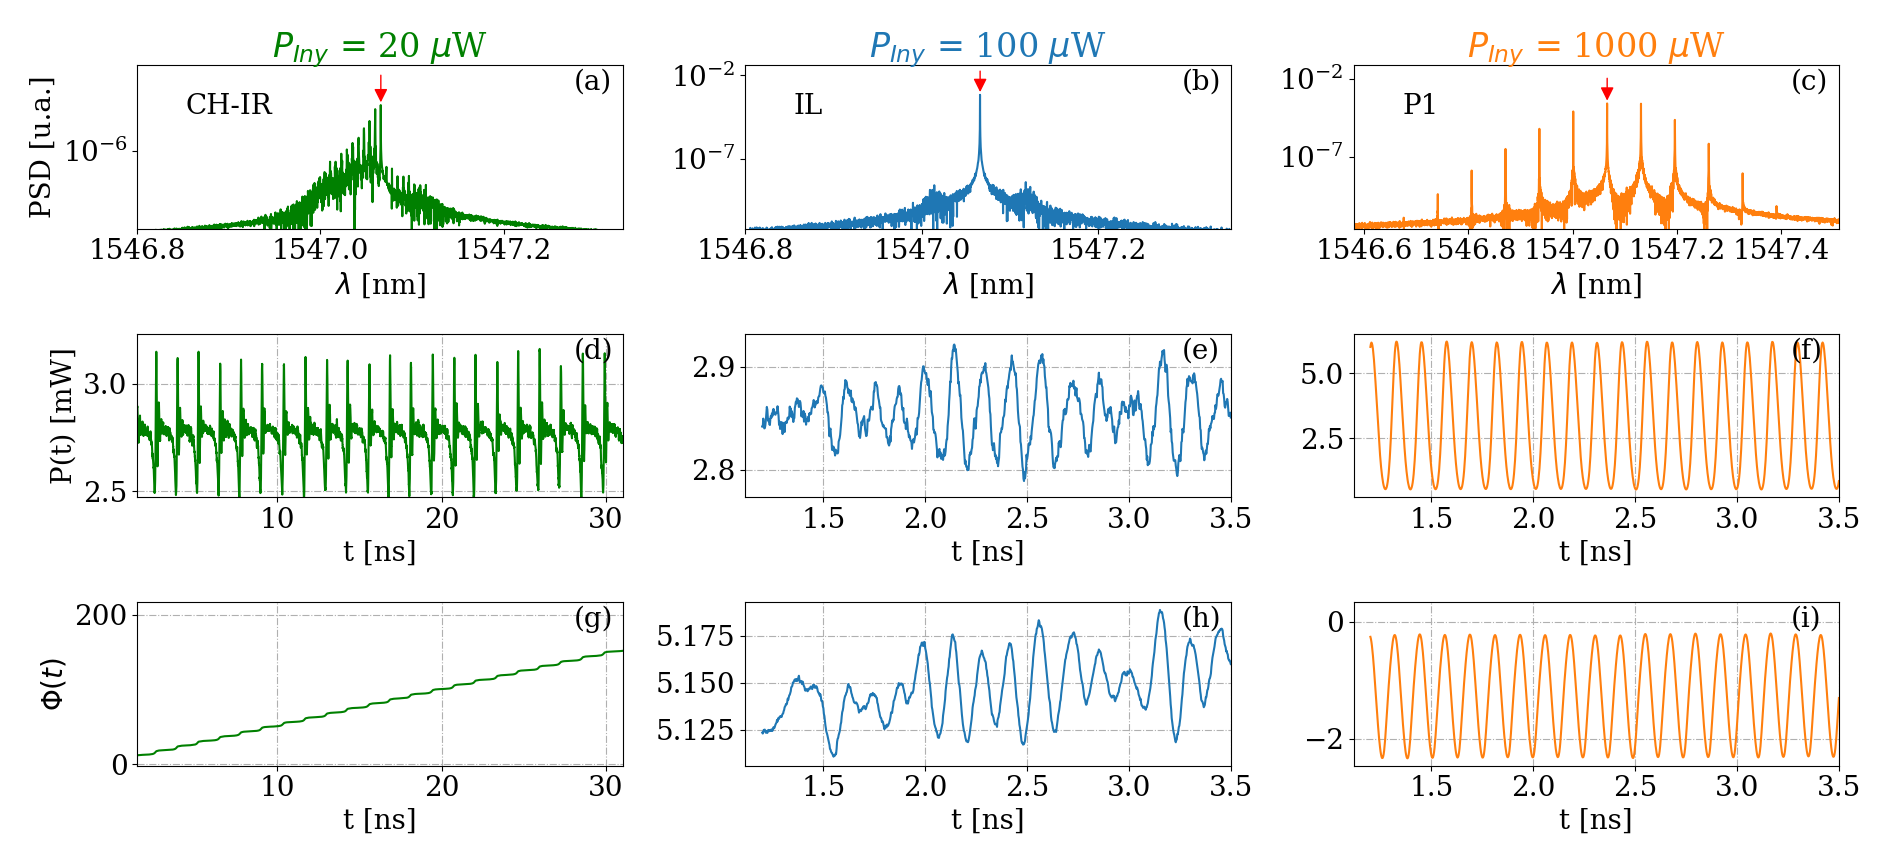
\includegraphics[width=1.0\linewidth]{zoneRtEq.png}
				\caption{\label{fig:zoneRtEq}ZoneRtEq}	
			\end{figure}

			\begin{figure}[H]
				\centering
				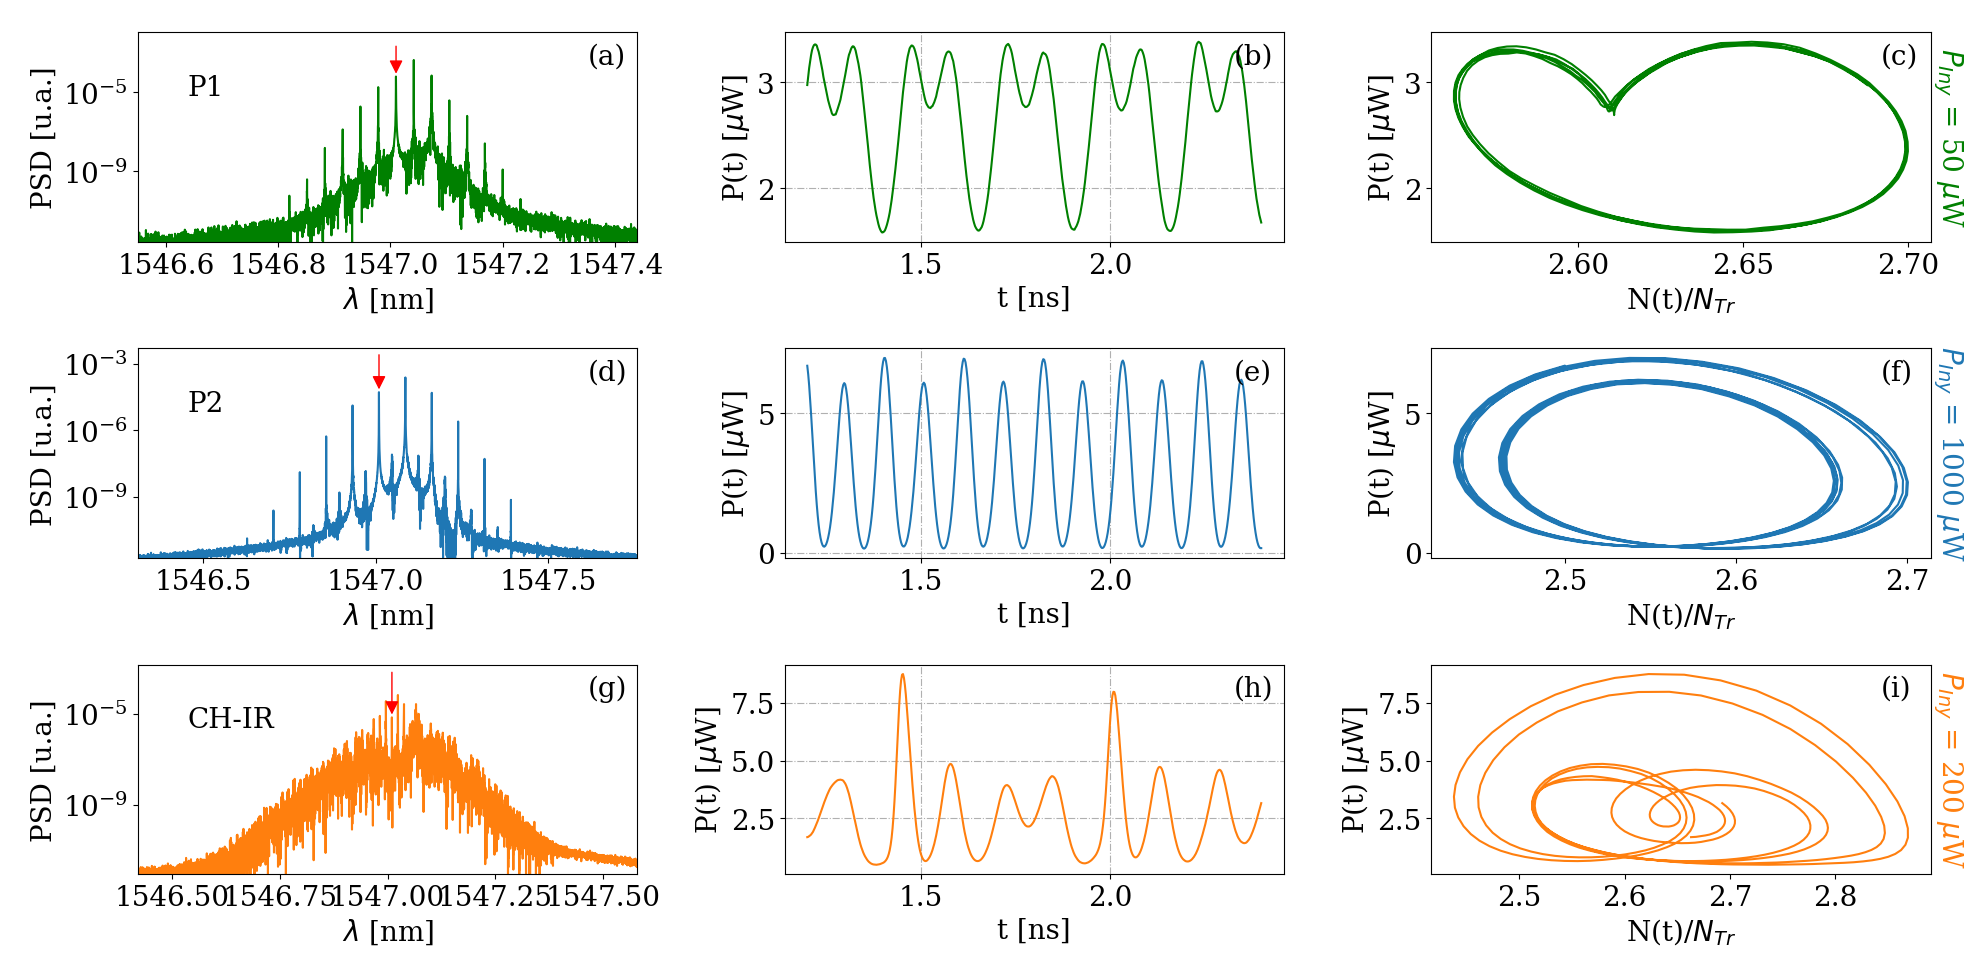
\includegraphics[width=1.0\linewidth]{P2zone.png}
				\caption{\label{fig:P2zone}P2zone}	
			\end{figure}


				
			\addtocontents{toc}{\vspace{0.1cm}}
			\chapter{Inyeccion de luz en OFC}

				\graphicspath{{../Graphics/Cpt3-CombInject/}}

En este cap\'itulo se han combinado los m\'etodos de generaci\'on de OFC estudiados en los cap\'itulos anteriores, abordando el estudio de los r\'egimenes din\'amicos que existen en la generaci\'on de OFC mediante \gs\ e inyecci\'on de luz. Se ha trabajado con el l\'aser ML con $\ibias = 35$ mA, $V_{RF} = 1.$ V y alta frecuencia $f_R = 5$ GHz. Para las condiciones de inyecci\'on de SL se ha tomado un \'unico valor de $\delta\nu = -2$ GHz, variando la potencia de inyecci\'on $P_{Iny}$.

En la Figura \ref{Img:MapGS-IO} se muestran los espectros \'opticos de las diferentes regiones din\'amicas obtenidas para distintas $P_{Iny}$ a $\delta\nu = -2$ GHz. 


			\begin{figure}[H]
				\centering
				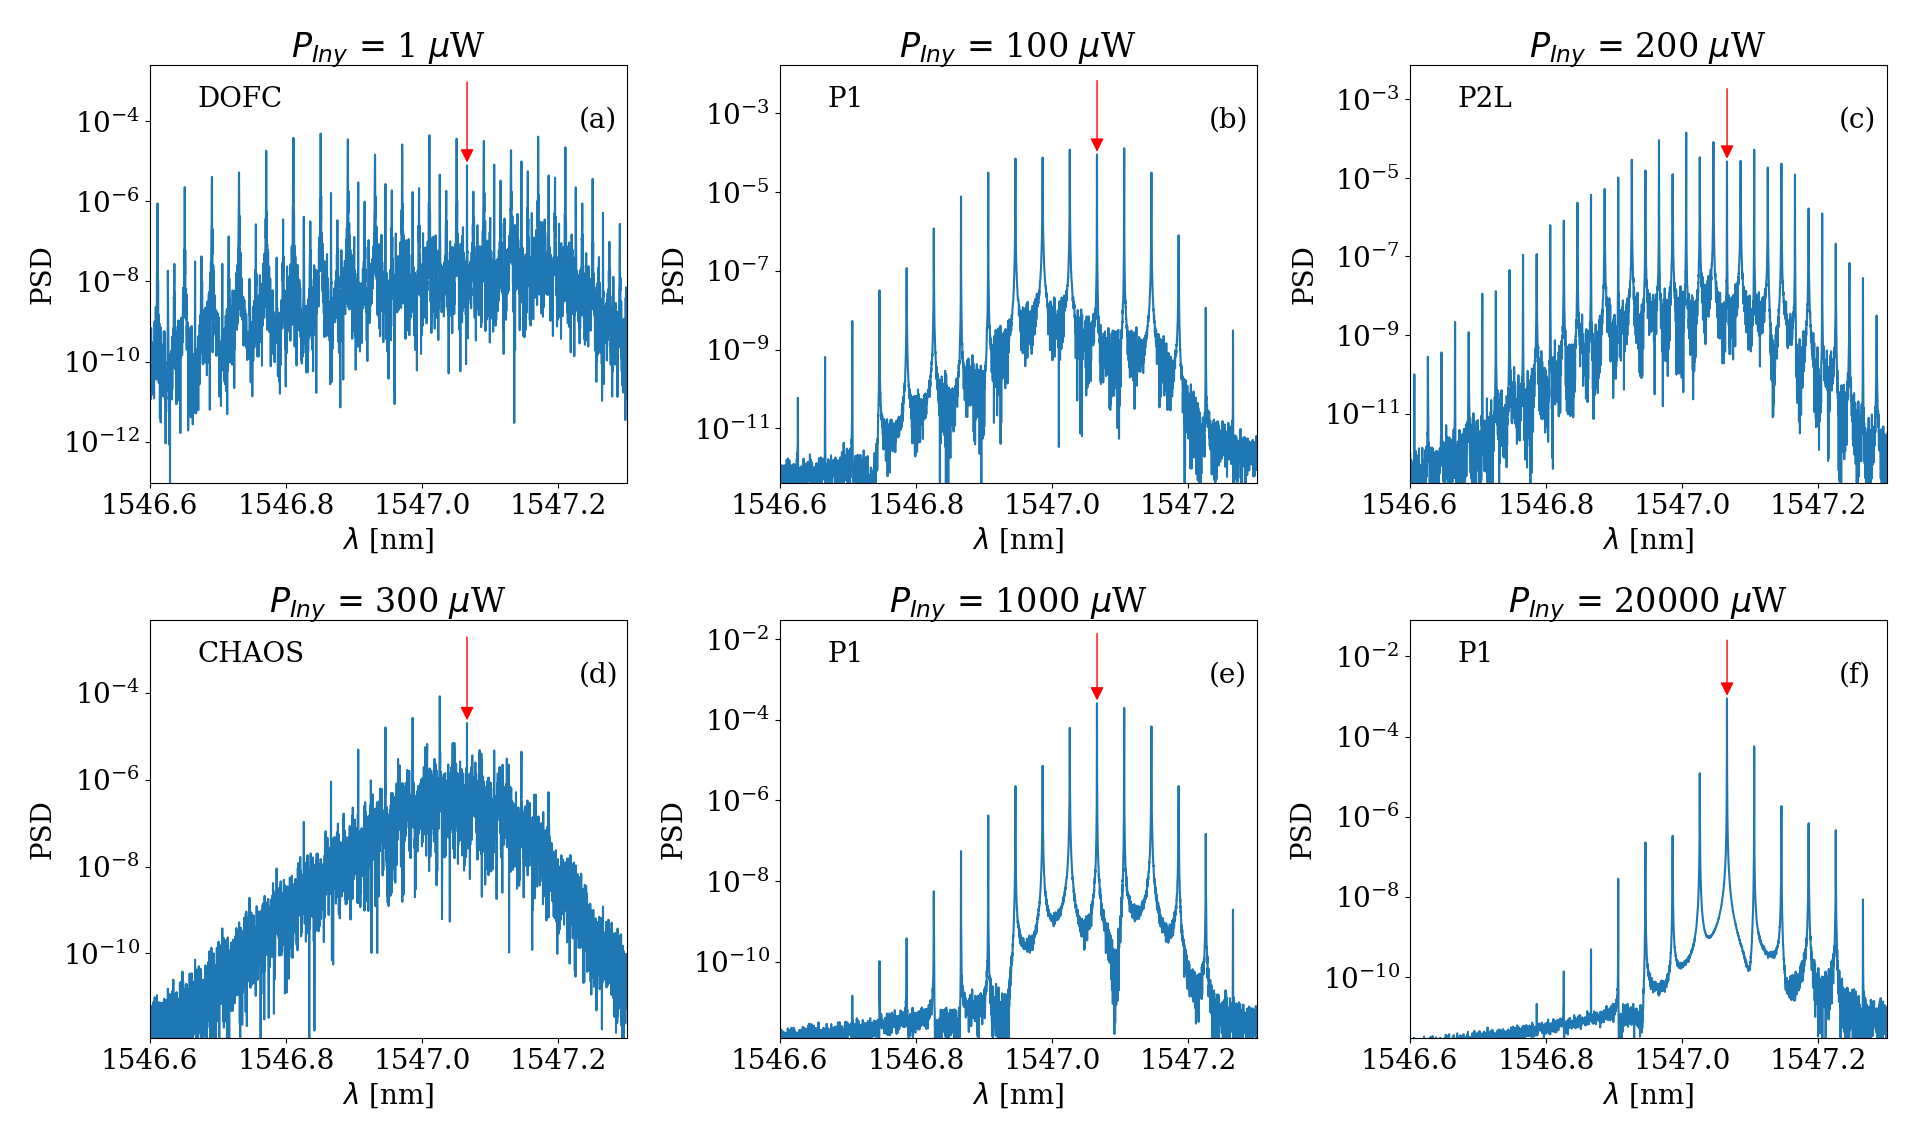
\includegraphics[width=1.0\linewidth]{psdMap.png}
				\caption{\label{Img:MapGS-IO}Espectros \'opticos obtenidos mediante \gs\ e inyección \'optica de las diferentes regiones dinámicas obtenidas para diferentes $P_{Iny}$ a $\delta\nu = -2$ GHz. Se indica la frecuencia de inyección $\nu_{SL}$ con una flecha y $P_{Iny}$ para cada espectro \'optico.}
			\end{figure}

		Para $P_{Iny} = 1\;\mu$W se obtiene un espectro \'optico con doble peine \'optico de frecuencias, DOFC, observando dos picos de emisión a cada lado del OFC principal (Figura \ref{Img:MapGS-IO} (a)). El DOFC se desruye al aumentar la potencia de inyección, obteniendo un OFC simple en la regi\'on P1 para $P_{Iny} = 100\;\mu$W (Figura \ref{Img:MapGS-IO} (b)). Al aumentar $P_{Iny} = 200 \;\mu$W se produce un doblamiento de periodo P2, obteniendo un OFC cuyas frecuencias de separaci\'on entre pico es la mitad que para la regi\'on P1 (Figura \ref{Img:MapGS-IO} (c)). La región de caos, CHAOS, se obtiene para $P_{Iny} = 300\;\mu$W, para la que el OFC se destruye (Figura \ref{Img:MapGS-IO} (d)). Con altas potencias de inyecci\'on $P_{Iny} = 1000\;\mu$W y $ 20000\;\mu$W se alcanza nuevamente la regi\'on P1 con un pico m\'aximo para la frecuencia de inyecci\'on $\nu_{SL}$. Dentro de esta regi\'on, al aumentar $P_{Iny}$ tanto el ruido debido a la emisi\'on espont\'anea como los picos de emisi\'on que se encuentran a los lados del pico en $\nu_{SL}$ disminuyen, mientras que el pico co nla frecuencia de inyecci\'on aumenta. Esta tendencia puede indicar la existencia de una nueva regi\'on con IL para $P_{Iny}$ superiores a los valores con los que se ha trabajado.

		Se han estudiado y comparado algunos casos concretos de las regiones mostradas en la Figura \ref{Img:MapGS-IO}, analizando el comportamiento de las variables internas con el objetivo de entender mejor los fen\'omenos que se producen en cada caso, de cara a realizar una correcta distinci\'on de las diferentes regiones din\'amicas.

		En la Figura \ref{fig:p1-p2} se muestran los espectros \'opticos, $P(t)$ y el atractor en el espacio de los estados de las ecuaciones de balance, despreciando los efectos de la fase \'optica; para $\delta\nu = -2$GHz y $P_{Iny} = 100\;\mu$W y $200\;\mu$W.

			\begin{figure}[H]
				\centering
				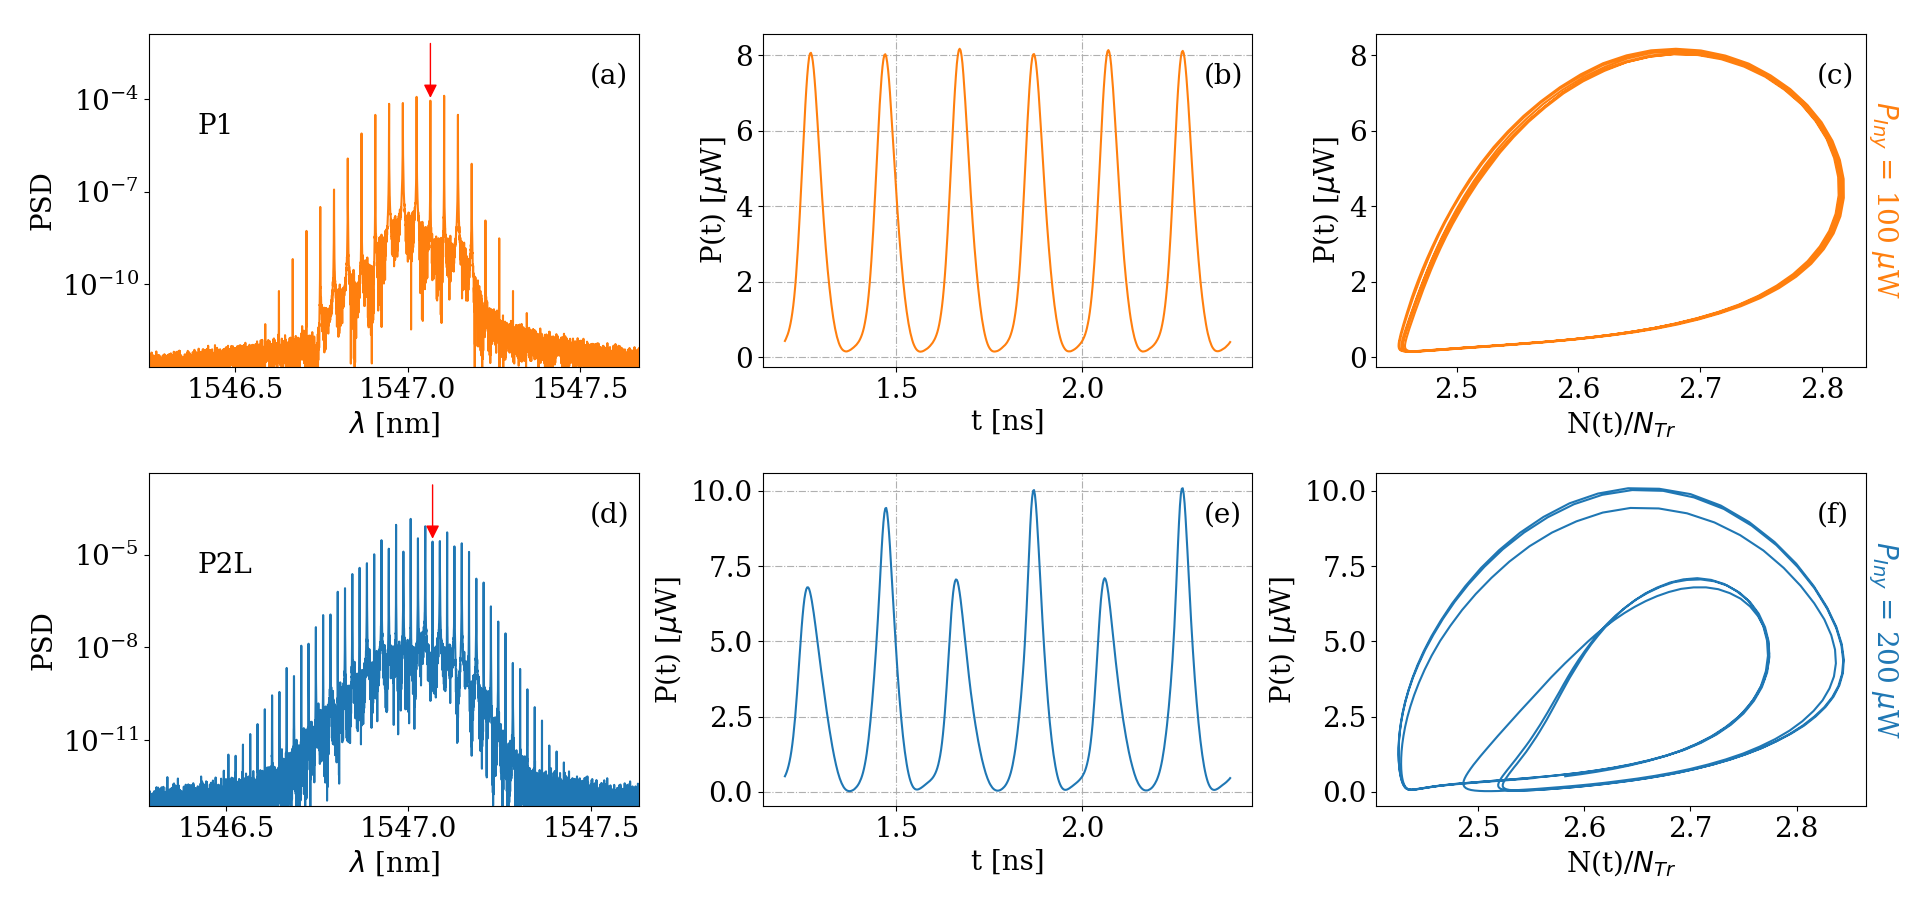
\includegraphics[width=1.0\linewidth]{p1-p2.png}
				\caption{\label{fig:p1-p2}Espectros \'opticos, $P(t)$ y atractor en el espacio de los estados de las ecuaciones de balance, despreciando los efectos de la fase \'optica; para $\delta\nu = -2$GHz y $P_{Iny} = 100\;\mu$W (P1, naranja) y $200\;\mu$W (P2, azul).}	
			\end{figure}

		Los resultados de la Figura \ref{fig:p1-p2} permiten comparar m\'s a fondo las regiones P1 y P2, obteniendo para ambos casos dos OFC con similares perfiles pero cuya separaci\'on entre l\'ineas es la mitad para el caso de P2. Esto se puede observar en la Figura \ref{fig:p1-p2} (e) en la que la diferencia de amplitudes entre picos continuos produce que el periodo de las oscilaciones de $P(t)$ no sea el tiempo entre picos continuas, sino el tiempo entre picos con la misma amplitud, que es el doble. Tambi\'en se puede observar en la Figura \ref{fig:p1-p2} (f) en la que se obtiene una doble oscilación con un diagrama similar al de la Figura \ref{fig:P2zon} (f) para la regi\'on P2 del c\'apitulo anterior.

		En la Figura \ref{fig:chaos} se muestran los espectros \'opticos, $P(t)$ y el atractor en el espacio de los estados de las ecuaciones de balance, despreciando los efectos de la fase \'optica; para $\delta\nu = -2$GHz y $P_{Iny} = 1\;\mu$W y $300\;\mu$W.

			\begin{figure}[H]
				\centering
				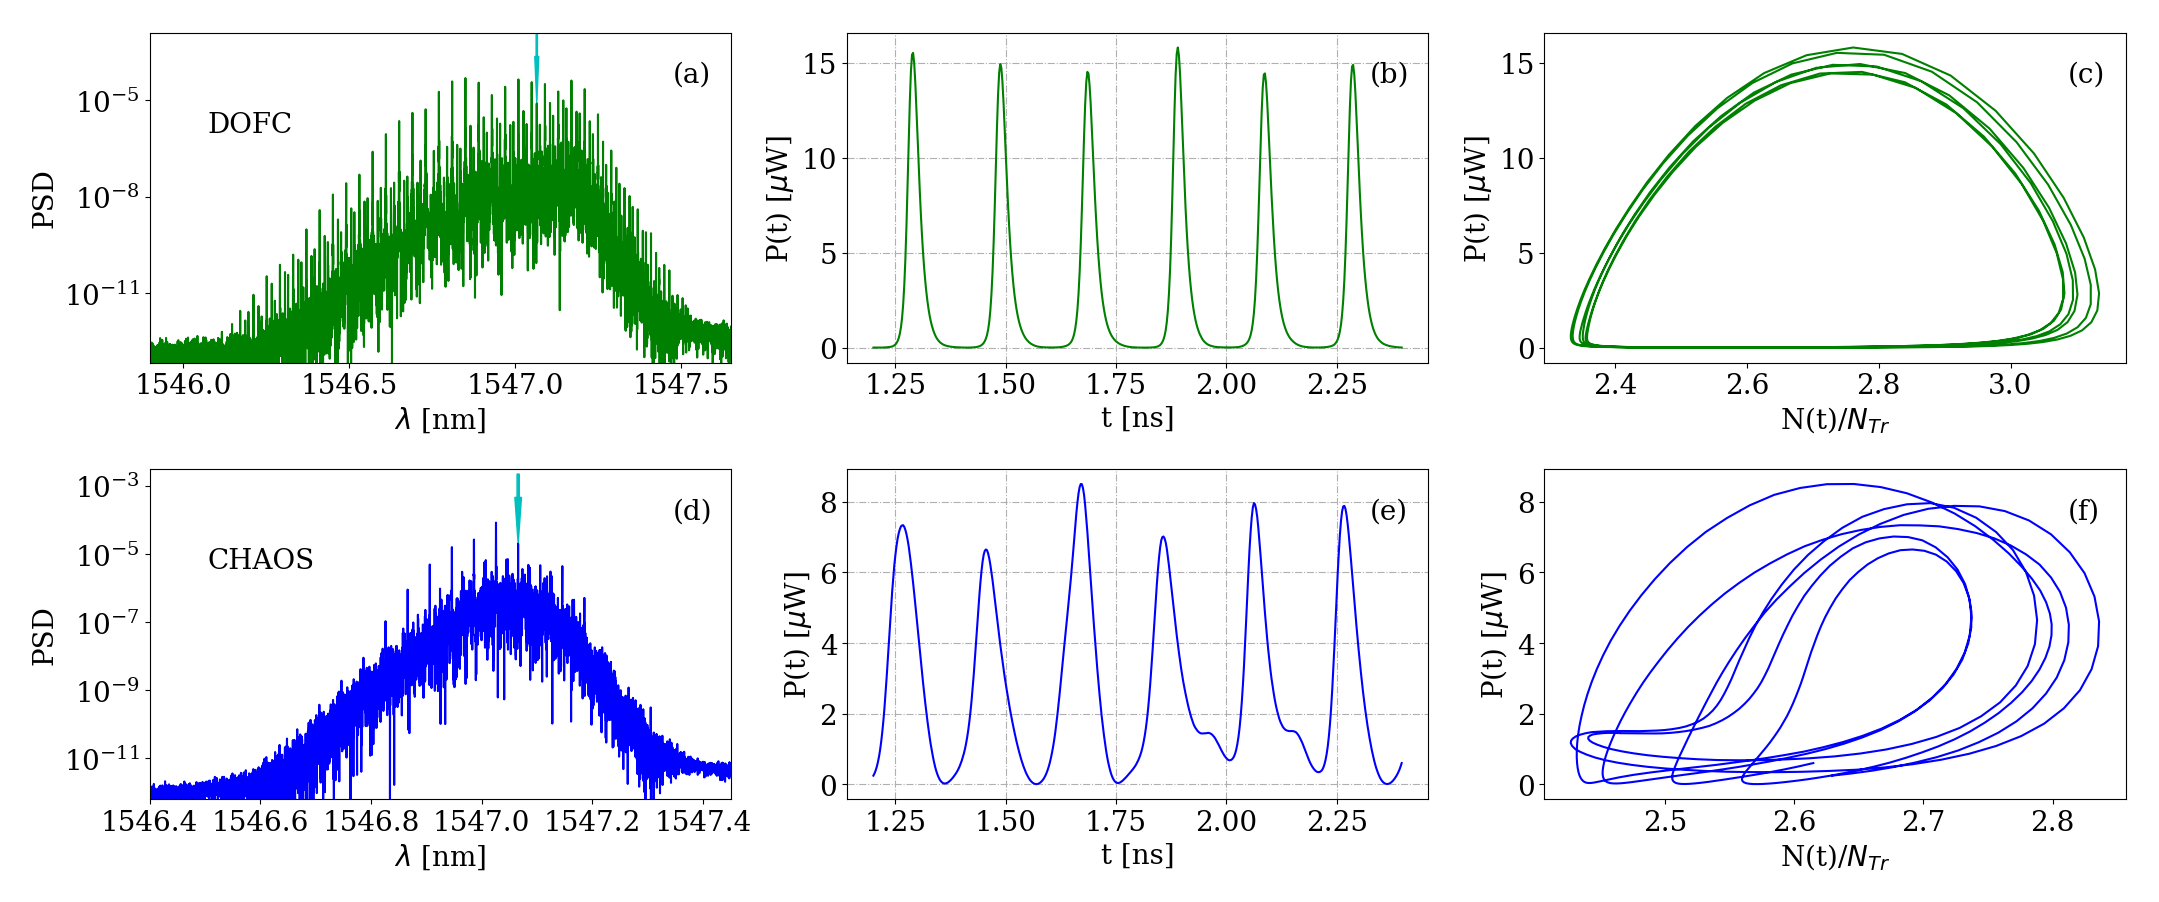
\includegraphics[width=1.0\linewidth]{chaos.png}
				\caption{\label{fig:chaos}Espectros \'opticos, $P(t)$ y atractor en el espacio de los estados de las ecuaciones de balance, despreciando los efectos de la fase \'optica; para $\delta\nu = -2$GHz y $P_{Iny} = 1\;\mu$W (DOFC, naranja) y $300\;\mu$W (CHAOS, azul).}	
			\end{figure}

		El espectro \'optico del DOFC (Figura \ref{fig:chaos} (a)) permite observar varias l\'ineas de emisión bien resultas y con una anchura entre ellas pequeña y bien definida. Ambos espectros \'opticos presentan un perfil similar formado por una ancha banda de ruido debido a la emisi\'on espont\'anea y l\'ineas de emisión que emergen de \'esta. Para el caso de CHAOS estos picos de emisi\'on son mucho menores que para el DOFC. La diferencia entre ambas regiones se hace m\'as notoria en la potencia $P(t)$, en la que para el caso del CHAOS (Figura \ref{fig:chaos} (e)) se observan oscilaciones con diferentes amplitudes para cada pido y diferentes tiempos entre \'estos. Los atractores obtenidos no dejan ninguna duda a la diferncia entre ambas regiones, obteniendo un diagrama tipo caos para $P_{Iny} = 300\;\mu$W en el que se tiende a tomar valores entodo el espacio de estados. Para el caso del DOFC se obtiene un diagrama de tipo P1 (Figura \ref{fig:chaos} (c) pero con algunas diferencias en los trazos.

%
				%\cite{rosado2018experimental}
%
			\addtocontents{toc}{\vspace{0.1cm}}
			\chapter{Conclusiones}

		%----------------------------------------------------------------------------------------
		%     BIBLIOGRAPHY
		%----------------------------------------------------------------------------------------

			\bibliographystyle{unsrt}
			\bibliography{biblio}

		%----------------------------------------------------------------------------------------
		%     APPENDIX
		%----------------------------------------------------------------------------------------
				
			\newpage

				\appendix

					\chapter{Código de la simulación}

						\definecolor{gray97}{gray}{.97}
\definecolor{gray75}{gray}{.75}
\definecolor{gray45}{gray}{.45}

\lstset{ frame=Ltb,
	framerule=0pt,
	aboveskip=0.1cm,
	framextopmargin=3pt,
	framexbottommargin=3pt,
	framexleftmargin=0.4cm,
	framesep=0pt,
	rulesep=.4pt,
	backgroundcolor=\color{gray97},
	rulesepcolor=\color{black},
	%
	stringstyle=\ttfamily,
	showstringspaces = false,
	basicstyle=\small\ttfamily,
	commentstyle=\color{gray45},
	keywordstyle=\bfseries,
	%
	numbers=left,
	numbersep=15pt,
	numberstyle=\tiny,
	numberfirstline = false,
	breaklines=true,
}

\lstdefinestyle{Python}
{basicstyle=\scriptsize\bf\ttfamily,
language=python,
}

\centering\small
\vspace{0.4cm} +- - - - - - - - - - - - - 18 l\'ineas - - - - - - - - - - - - -+
\lstinputlisting[style=Python, firstline=19, lastline=26, firstnumber=19]{../src/simulation.py}
\vspace{-0.4cm} +- - - - - - - - - - - - - 18 l\'ineas - - - - - - - - - - - - -+
\lstinputlisting[style=Python, firstline=44, lastline=53, firstnumber=44]{../src/simulation.py}

\vspace{-0.4cm} +- - - - - - - - - - - - - 24 l\'ineas - - - - - - - - - - - - -+
\lstinputlisting[style=Python, firstline=77, lastline=81, firstnumber=77]{../src/simulation.py}

\vspace{-0.4cm} +- - - - - - - - - - - - - 15 l\'ineas - - - - - - - - - - - - -+
\lstinputlisting[style=Python, firstline=96, lastline=96, firstnumber=96]{../src/simulation.py}

\vspace{-0.4cm} +- - - - - - - - - - - - - 20 l\'ineas - - - - - - - - - - - - -+
\newpage
\lstinputlisting[style=Python, firstline=116, lastline=155, firstnumber=116]{../src/simulation.py}

\vspace{-0.4cm} +- - - - - - - - - - - - - 10 l\'ineas - - - - - - - - - - - - -+
\newpage
\lstinputlisting[style=Python, firstline=165, lastline=192, firstnumber=165]{../src/simulation.py}

\vspace{-0.4cm} +- - - - - - - - - - - - - 10 l\'ineas - - - - - - - - - - - - -+
\lstinputlisting[style=Python, firstline=202, lastline=206, firstnumber=202]{../src/simulation.py}

\vspace{-0.4cm} +- - - - - - - - - - - - -  6 l\'ineas - - - - - - - - - - - - -+
\lstinputlisting[style=Python, firstline=212, lastline=220, firstnumber=212]{../src/simulation.py}

\vspace{-0.4cm} +- - - - - - - - - - - - - 39 l\'ineas - - - - - - - - - - - - -+
%\lstinputlisting[style=Python, firstline=96, lastline=220, firstnumber=100]{../src/simulation.py}


	\end{document}

%----------------------------------------------------------------------------------------
%              END
%----------------------------------------------------------------------------------------
